	\section{Il ciclo di vita del Data Warehouse}
Trattandosi di sistemi complessi è fondamentale seguire una metodologia. Questi progetti hanno diversi fattori di rischio:
\begin{itemize}
	\item
	Rischi legati alla gestione del progetto
	\item 
	Rischi legati alle tecnologie
	\item 
	Rischi legati ai dati e alla progettazione
	\item 
	Rischi legati all'organizzazione
\end{itemize}
Esistono due macro-approcci di progettazione:
\begin{itemize}
	\item 
	\textbf{Top-down}: significa pensare, concepire, progettare e costruire il DW come un monolite, cioè considerando i bisogni di tutta l’azienda in modo da coprirli per intero. In linea di principio, questo è un metodo eccezionale, perché si basa su una visione globale e garantisce di ottenere una perfetta integrazione consistente tra i reparti. Questo comporta fare un’analisi con tutti gli utenti dell’azienda e  capire come sono fatti tutti i DB aziendali. Questo può portarmi alla paralisi dell’analisi, cioè  arrivare in una situazione in cui il costo dell’analisi diventa eccessivo. Inoltre, è difficile prevedere a priori le esigenze di tutti gli utenti. Il fatto di non prevedere una consegna a breve termine non permette agli utenti di verificare l’utilità del progetto e ne fa scemare l’interesse e la fiducia. 
	\item 
	\textbf{Bottom-up}: costruire il DW in modo incrementale, un pezzo alla volta. Solo alla fine ho la visione globale del DW. Il pezzo utilizzato nel metodo incrementale è proprio il data mart. L’idea di questo approccio è pensare, progettare ed implementare un data mart alla volta. Ciò determina risultati concreti in tempi brevi. Il progettista deve fare analisi dei requisiti solo su un ‘area aziendale e per alimentare quel data mart non ho bisogno di tutti i DB aziendali, ma solo di qualcuno. Altro vantaggio è quello di mantenere elevato l’attenzione degli utenti sul progetto.
\end{itemize}

Il primo passo per la realizzazione di un DW è scegliere il primo data mart, il quale deve essere strategico, cioè coprire un ruolo centrale e di riferimento per l’intero DW. Si deve appoggiare su fonti dati già disponibili e consistenti. 

A livello macroscopico il ciclo di sviluppo può essere rappresentato dalla figura \ref{fig:ciclo}. 
\begin{figure}[H]
	\centering
	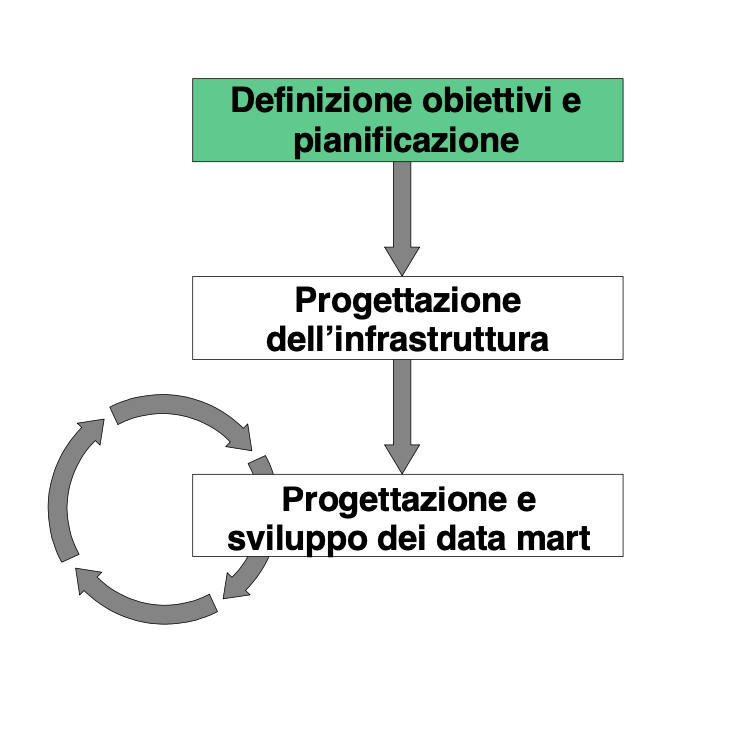
\includegraphics[width=0.5\linewidth]{img/cicloDW}
	\caption{Ciclo DW}
	\label{fig:ciclo}
\end{figure}
Vi è una prima di fase di definizione degli obiettivi e dei confini, in cui si prepara una roadmap di progetto per il medio lungo termine. Questa fase comporta la scelta dell’architettura. 

La seconda fase è di progettazione dell’infrastruttura e prevede la scelta dello stack tecnologico. Molte volte questa scelta non risulta essere libera perché ci si basa sulle tecnologie che già si hanno in casa e anche per avere meno problemi di interoperabilità tra i software. 

L’ultima fase è la fase iterativa, in cui ad ogni giro, si realizza un nuovo data mart che viene integrato nel sistema di DW. 
\subsection{Progettazione del data mart}
La progettazione di data mart coinvolge diverse figure, quali il progettista, l’amministratore di db e l’utente finale, ed è composta da diverse fasi:
\begin{itemize}
	\item
	\textbf{Analisi e riconciliazione delle sorgenti}: l’idea è capire come sono fatte le basi di dati utilizzate come sorgenti per alimentare il data mart. Le sorgenti dati sono analizzate, normalizzate e integrate per ottenere uno schema riconciliato per l’ODS
	\item 
	\textbf{Analisi dei requisiti}: capire che cosa gli utenti devono fare con questo sistema, cioè quali fatti devono modellare, con quali dimensioni, con quali misure, in modo da ottenere report e risultati di analisi. Questa fase avviene attraverso delle interviste
	\item
	\textbf{Progettazione concettuale}: rappresenta i concetti che devono essere gestiti nel DB in maniera indipendente dall’implementazione. In questo caso significa disegnare uno schema concettuale del data mart, cioè uno schema che spiega il contenuto informativo ma senza entrare nel merito dell’implementazione. Lo schema concettuale per essere corretto dovrà tener conto dei dati sorgenti e rispettare i requisiti utente. 
	\item 
	\textbf{Carico di lavoro e volume dati}: insieme delle query che verranno sottoposte al sistema. Si profilano gli utenti (coordinatore corso di studi, preside ecc.) e infine si misura il volume dati.
	\item 
	\textbf{Progettazione logica}: riprendo lo schema concettuale e lo traduco in uno schema logico, il che è dipendente dall’implementazione, in cui scelgo il tipo di piattaforma implementativa (ROLAP o MOLAP). 
	\item 
	\textbf{Progettazione dell’ETL}: si progettano le procedure ETL, le quali come abbiamo già detto, hanno il compito di “rinfrescare” i contenuti del data mart tenendo conto delle modifiche fatte nel DB sorgente.
	\item
	\textbf{Progettazione fisica}: non mi basta aver scelto l’implementazione, ma devo sapere anche qual è lo stack tecnologico. Devo tipicamente creare gli indici, e poiché ogni specifico DBMS ha le sue regole, in questa fase devo sapere su quale stack tecnologico mi devo muovere.
	\item 
	\textbf{Implementazione della reportistica}: si creano i report a partire dal carico di lavoro. Resto sul front-end che ho scelto, creo i meta dati e devo creare i report. 
	\item 
	\textbf{Testing}: si testano le procedure ETL e i report
\end{itemize}
Le diverse fasi possono incastrarsi in maniera diversa e a seconda del quadro metodologico che adotto:
\begin{itemize}
	\item 
	\textbf{Approccio guidato dai dati (supply-driven)}: la forma dei DB sorgente mi guida nella progettazione del data mart. I requisiti utente impattano sul progetto guidando il progettista nella selezione delle porzioni di dati considerate rilevanti per il processo decisionale, e determinando la loro strutturazione secondo il modello multidimensionale
	\item 
	\textbf{Approccio guidata dai requisiti (demand-driven)}: quello che mi traina nella progettazione sono i requisiti dell’utente
\end{itemize}
\subsubsection{Supply-Driven}
Come riportato in figura \ref{fig:supply} inizio con il guardare il contenuto delle sorgenti. Le sorgenti sono caratterizzate attraverso i loro schemi. Nel caso di DB relazionale ho lo schema logico o un entity-relation. L’analisi e la riconciliazione nello specifico prevede l’integrazione degli schemi in modo da avere in uscita uno schema riconciliato, che mi restituisce una visione unica di quella fetta di dato. In un’architettura a tre livelli, quello schema diventa lo schema dell’ODS. Quindi effettuo l’analisi dei requisiti
attraverso le interviste e in un’uscita si possono usare dei glossari tenendo traccia delle cose principali che mi hanno detto gli utenti. Quindi posso passare alla progettazione concettuale, prendendo lo schema riconciliato e ottenendo uno schema per i data mart, detto schema di fatto. Intanto lavoro sul carico di lavoro e volume dati, scrivendomi le query più frequenti e la reportistica che potrebbe servire. Adesso si è pronti per fare la progettazione logica, si prende lo schema di fatto e tenendo conto di carico e lavoro di volume dati, lo si traduce in uno schema logico. A questo punto posso passare alla progettazione dell’ETL e infine alla progettazione fisica, scegliendo il DBMS e ottenendo dallo schema logico lo schema fisico. 
\begin{figure}[H]
	\centering
	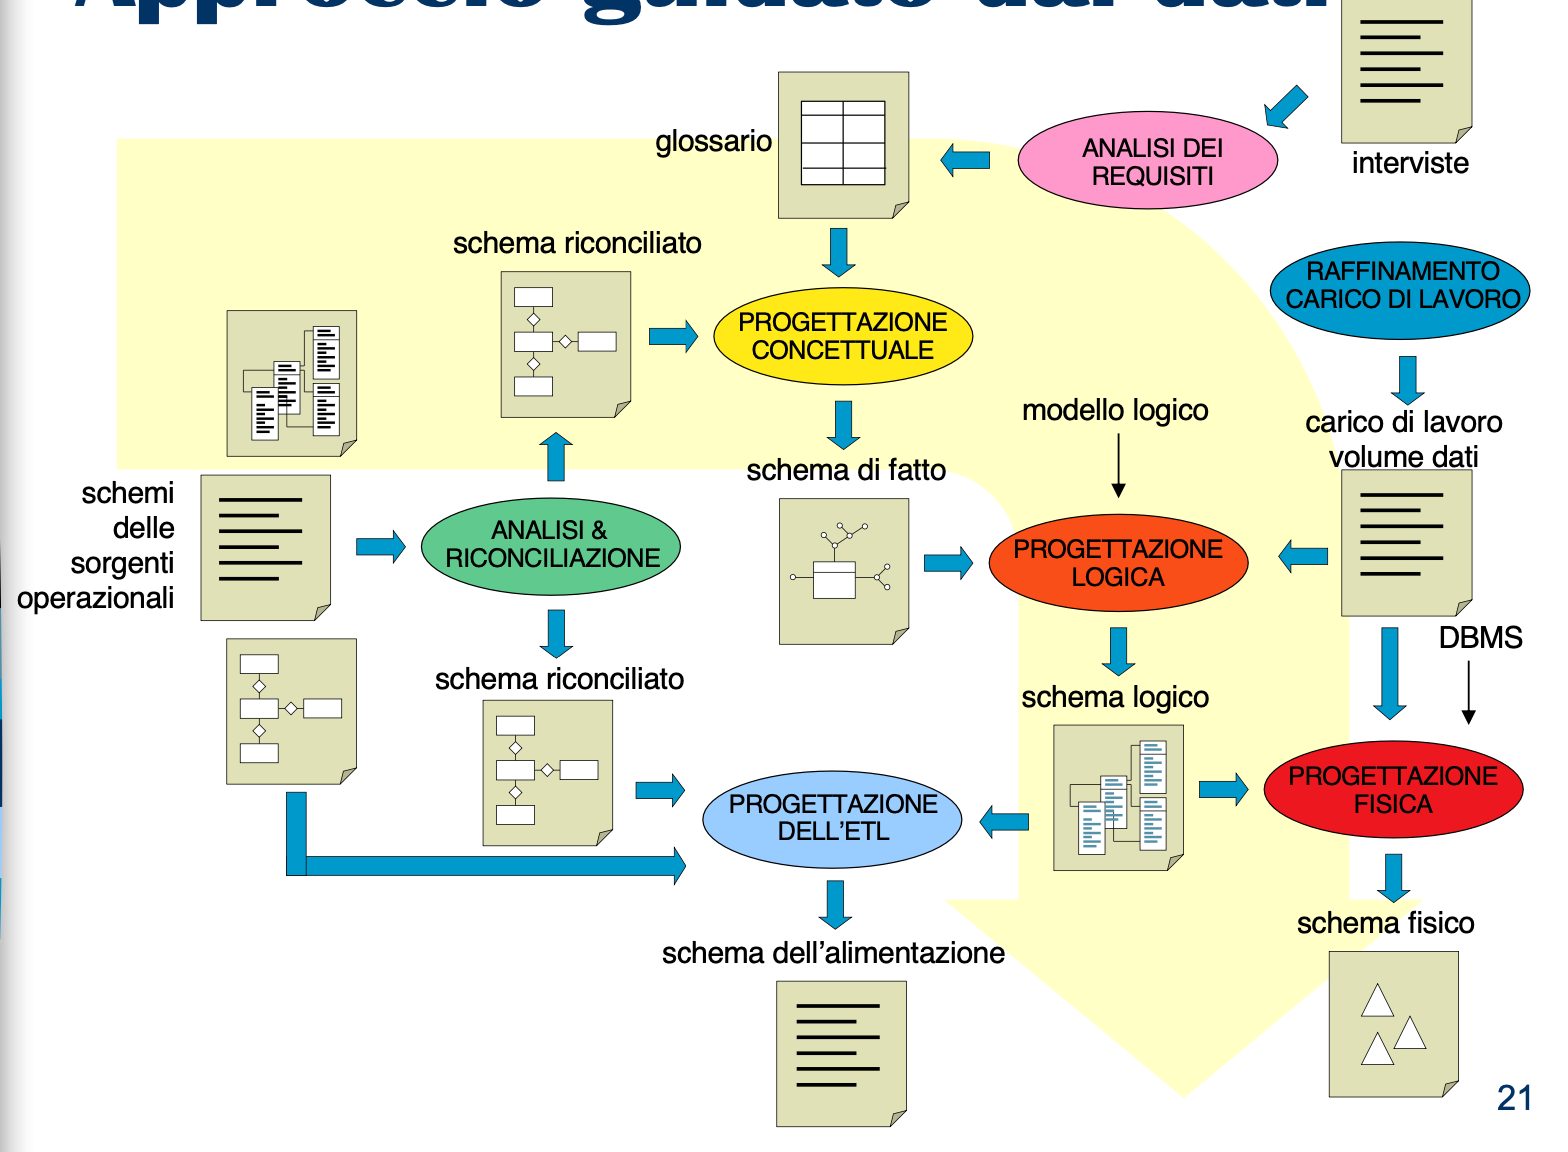
\includegraphics[width=0.7\linewidth]{img/supply-driven}
	\caption{Supply-Driven}
	\label{fig:supply}
\end{figure}
\textbf{Vantaggi}

Il grosso vantaggio è l’esistenza di un algoritmo che banalizza la fase di progettazione concettuale a partire dai dati riconciliati. 

L’algoritmo come prodotto laterale restituisce i mapping tra i concetti del data mart e i concetti dello schema sorgente. 

\textbf{Svantaggi}

Ai requisiti utente viene assegnato un ruolo secondario nel determinare i contenuti informativi per l’analisi, mentre al progettista viene dato un supporto limitato per l’identificazione di fatti, dimensioni e misure.

\textbf{Applicabilità}

Tale approccio è applicabile quando:
\begin{itemize}
	\item 
	Conosca in anticipo gli schermi delle sorgenti e questi siano normalizzati e non complessi, perché quest’algoritmo si nutre di dipendenze funzionali, cioè funziona andando a leggere le dipendenze funzionali codificate nel DB sorgente
	\item 
	Quando l’architettura prescelta prevede l’adozione di un livello riconciliato questi requisiti sono soddisfatti: la normalizzazione e la conoscenza approfondita sono garantite dalla riconciliazione. Lo stesso vale nel caso in cui la sorgente si riduca ad un singolo Database, ben progettato e di dimensioni limitate
	\item
	Risulta essere l’approccio preferibile perché meno soggetto a errori ed estremamente più veloce del demand-driven.
\end{itemize}

\subsubsection{Demand-Driven}
Nel secondo tipo di approccio si parte dall’analisi dai requisiti e sulla base dei requisiti utente disegno lo schema concettuale. Una volta effettuata anche la fase del carico di lavoro posso passare alla progettazione logica, in modo da creare lo schema del DB del data mart sulla base dei requisiti utente. Passo alla progettazione dell’ETL partendo dagli schemi sorgenti, ma adesso questo risulta essere più costoso. Infine, passo alla progettazione fisica.\\

\textbf{Vantaggi}

I desideri degli utenti vengono portati in primo piano

\textbf{Svantaggi}

È richiesto al progettista uno sforzo consistente durante il disegno dell’alimentazione. Dunque fatti, misure e gerarchie vengono ricavate direttamente dalle specifiche dettate dagli utenti, e solo a posteriori si verifica che le informazioni richieste siano effettivamente disponibili nei database operazionali. In questo modo però la fiducia del cliente verso il progettista e verso l’utilità del data mart può venir meno

\textbf{Applicabilità}

Questo approccio costituisce l’unica alternativa nei casi in cui non sia fattibile a priori un’analisi approfondita delle sorgenti (per esempio quando il data mart viene alimentato da un sistema ERP), oppure qualora le sorgenti siano rappresentate da sistemi legacy di tale complessità da sconsigliarne la ricognizione e la normalizzazione. 

\subsection{Fasi di progettazione del data mart}
\subsubsection{Analisi e riconciliazione delle sorgenti}
L’obiettivo è fare l’integrazione del DB per ottenere l’ODS. Questa è la fase che ragiona principalmente sugli schemi, cioè la componente intensionale del DB. Quello che otteniamo in uscita da questa fase è l’ODS. 
Quando invece si dovrà disegnare l’ETL non basta lo schema ma bisogna ragione anche con i dati. 

Supponiamo di avere due database sorgenti, dove per ciascuno devo attuare una fase di ricognizione e normalizzazione. In input su ciascun DB sorgente ho uno schema logico e in uscita da ciascuno di queste due fasi ho uno schema concettuale trasformato che metto insieme ottenendo uno schema concettuale globale e riconciliato perché ha sanato gli eventuali conflitti. 
\begin{figure}[H]
	\centering
	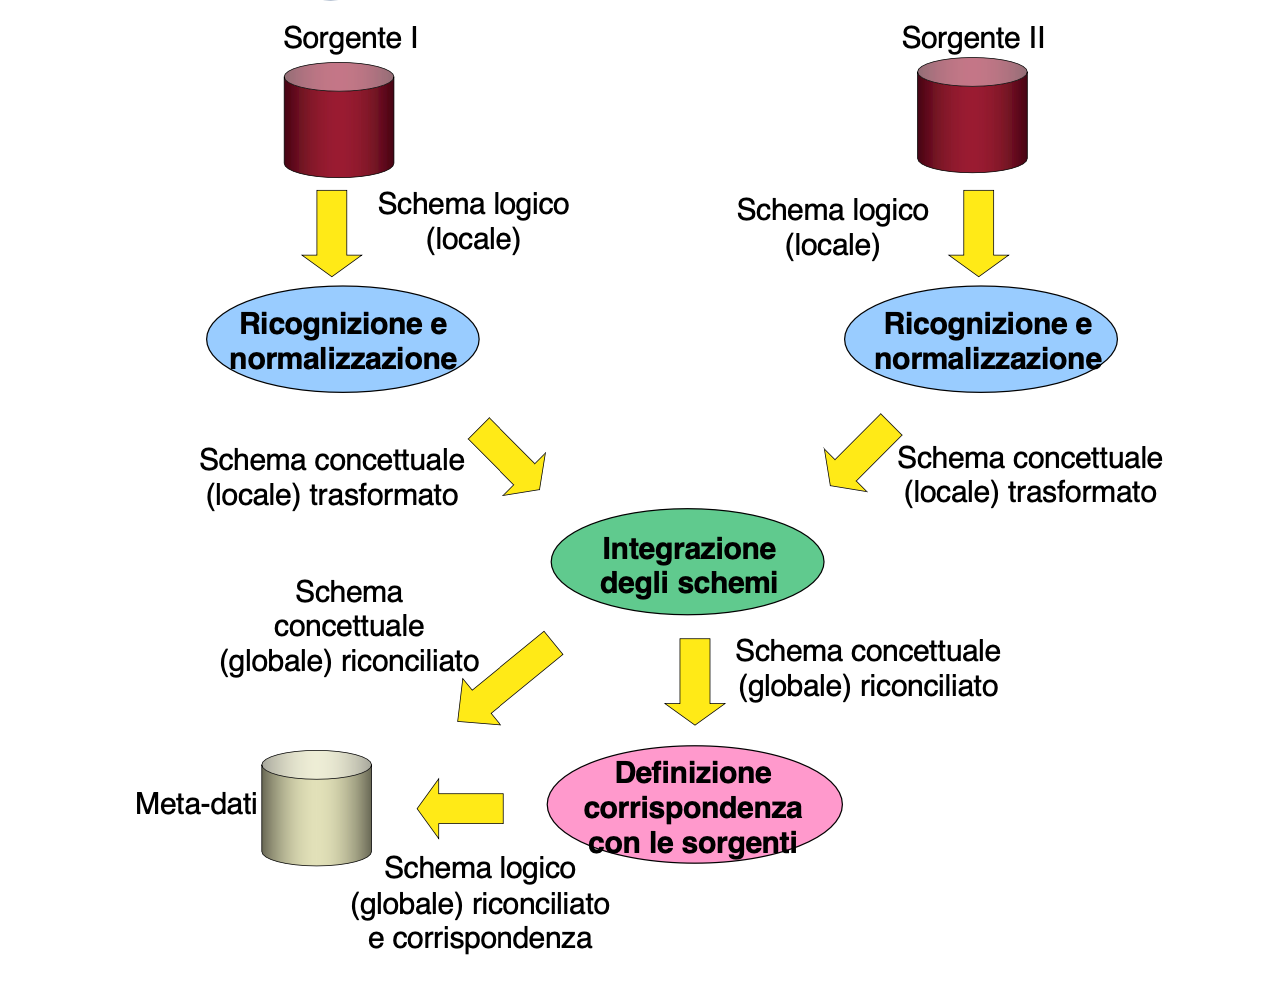
\includegraphics[width=0.7\linewidth]{img/analisi}
	\caption{Fase di analisi e riconciliazione}
	\label{fig:analisi}
\end{figure}
\subsubsection{Ricognizione e Normalizzazione}
\begin{itemize}
	\item
	\textbf{Ricognizione}: analisi approfondito degli schemi locali, guardo le tabelle e cerco di capire il significato di ciascuna tabella
	\item 
	\textbf{Normalizzazione}: significa che in teoria dovrei accorgermi che ci sono delle tabelle denormalizzate, cioè che ci sono delle dipendenze funzionali nascoste. 
\end{itemize}

\subsubsection{Analisi dei requisiti}
Qui l’obiettivo è raccogliere le esigenze di utilizzo del data mart espresse dai suoi utenti finali. Essa ha un’importanza fondamentale:
\begin{enumerate}
	\item 
	Perchè impatta in primis sullo schema concettuale
	\item 
	Specifiche per l'ETL legata alla sporcizia dei dati
	\item 
	Specifiche per l'analisi dei dati
\end{enumerate}
Ho due principali categorie di utenti:
\begin{itemize}
	\item 
	\textbf{Business Users}: persone che non sono tecniche. Usano il loro linguaggio, contraddicendosi tra di loro ma anche con sé stessi
	\item 
	\textbf{DBA}: in questo caso, i requisiti che dovranno essere catturati riguardano principalmente vincoli di varia natura imposti sul sistema di DW.
\end{itemize}
Per l’analisi dei requisiti bisogna preparare delle interviste indicendo delle riunioni, durante la quale si parla con i clienti. Ci sono due modi per strutturare un’intervista:
\begin{itemize}
	\item 
	\textbf{A piramide}: è un approccio di tipo induttivo, in cui l’intervistatore parte da domande molto dettagliate e progressivamente si allarga l’ambito della domanda. Questo tipo di approccio va bene con un intervistato scettico, che non si vuole far coinvolgere.
	\item
	\textbf{A imbuto}: si parte da domande più ampie e via via con domande più specifiche. Viene usato con un intervistato che è in soggezione. 
\end{itemize}
In qualunque modo si faccia l’analisi dei requisiti la cosa fondamentale è arrivare ad aver capito quali sono i fatti, in quando il fatto è la granularità (livello più spinto di dettaglio a cui voglio arrivare) giusta dell’informazione da catturare. A volte gli analisti fanno delle riunioni di analisi guidate dalle query, creando dei problemi, perché se chiedo agli utenti le query che vogliono fare, ottengo molte query e di conseguenza risulta difficile ottenere i fatti. Per ogni fatto occorre definire l’intervallo di storicizzazione, ovvero l’arco temporale che gli eventi memorizzati devono coprire. 
\subsubsection{Il carico di lavoro}
Il carico di lavoro OLAP è imprevedibile, ma è anche vero che il nucleo del carico di lavoro lo posso prevedere, perché ho già la reportistica statica, oltre quei report che l’utente ha già e che devono essere replicati nel nuovo cubo. In questa fase il carico di lavoro può essere espresso in linguaggio naturale; esso sarà comunque utile per valutare la granularità dei fatti e le misure d’interesse, nonché per iniziare ad affrontare il problema dell’aggregazione. 

Altri requisiti che vanno colti durante la fase di analisi sono legati alla periodicità dell’alimentazione (ogni quando deve fare l’ETL?) 